\documentclass[graphics]{beamer}

\usepackage{graphicx}
\usepackage{verbatim}
\usepackage{wrapfig}
\useoutertheme{shadow}
%\usecolortheme{orchid}
\usecolortheme{seahorse}


% math commands
\newcommand{\be}{\begin{eqnarray}}
\newcommand{\ee}{\end{eqnarray}}
\newcommand{\beq}{\begin{equation}}
\newcommand{\eeq}{\end{equation}}
\def\simless{\mathbin{\lower 3pt\hbox
      {$\rlap{\raise 5pt\hbox{$\char'074$}}\mathchar"7218$}}}
\def\simgreat{\mathbin{\lower 3pt\hbox
      {$\rlap{\raise 5pt\hbox{$\char'076$}}\mathchar"7218$}}} %> or of order

% variables

\def\toonscale{0.45}
\def\mboxy#1{\mbox{\small #1}}


\begin{comment}
\AtBeginSection[]{
  \frame{
    \frametitle{Outline}
    \tableofcontents[currentsection]
  }
}
\end{comment}

\title{21cm absorbers
}
%\subtitle{interim update}
\author[U. Pen]{Ue-Li Pen
\\[8mm] 
}
\date{May 18, 2021}


\begin{document}

%\section*{Introduction}
\section{Absorbers}

\begin{comment}
  \subsection{Outline}

  \frame{
    \frametitle{Outline}
    \tableofcontents
  }
\end{comment}

\frame{\maketitle}



  \frame{
    \frametitle{21cm Absorbers}
    \begin{itemize}
        \item 21cm transition: $\Delta T=h\nu/k=68$mK
        \item $\Delta T \ll 2.78$K:  $3n_1/n_0=\exp(\delta E/kT)\sim
          1+0.068/T$
          \item optical depth $\tau \propto 1/T$
        \item emission $\propto T\tau$ is independent of T, absorption $\propto 1/T$
        \item coldest atoms in LoS dominate
        \item typically dominated by cold atomic clouds
    \end{itemize}
  }


  \frame{
\vspace{-0.5in}
    \frametitle{History}
    \begin{itemize}
    \item 21cm absorber first detected in 3C286 at GBO in 1970's (Brown+Roberts 1973)
        \item current best constraint on direct measurement of cosmic
          acceleration (Darling 2012)
\item $z= 0.692153275(85)$, with $\dot{ż} = (1.6 \pm 4.7) \times 10^{-8}$/yr,
  expected $\dot{z}=2\times 10^{-11}$/yr using only 8 year baseline
        \item concept: watch the doppler shift of objects change with
          time:
          \item acceleration: doppler shift increases with time
          \item deceleration: doppler shift decreases with time
          \item bypasses need of general relativity: circular question
            if Dark Energy is on the RHS?
                \end{itemize}
  }


  \frame{
\vspace{-0.5in}
    \frametitle{Counts}
\begin{center}
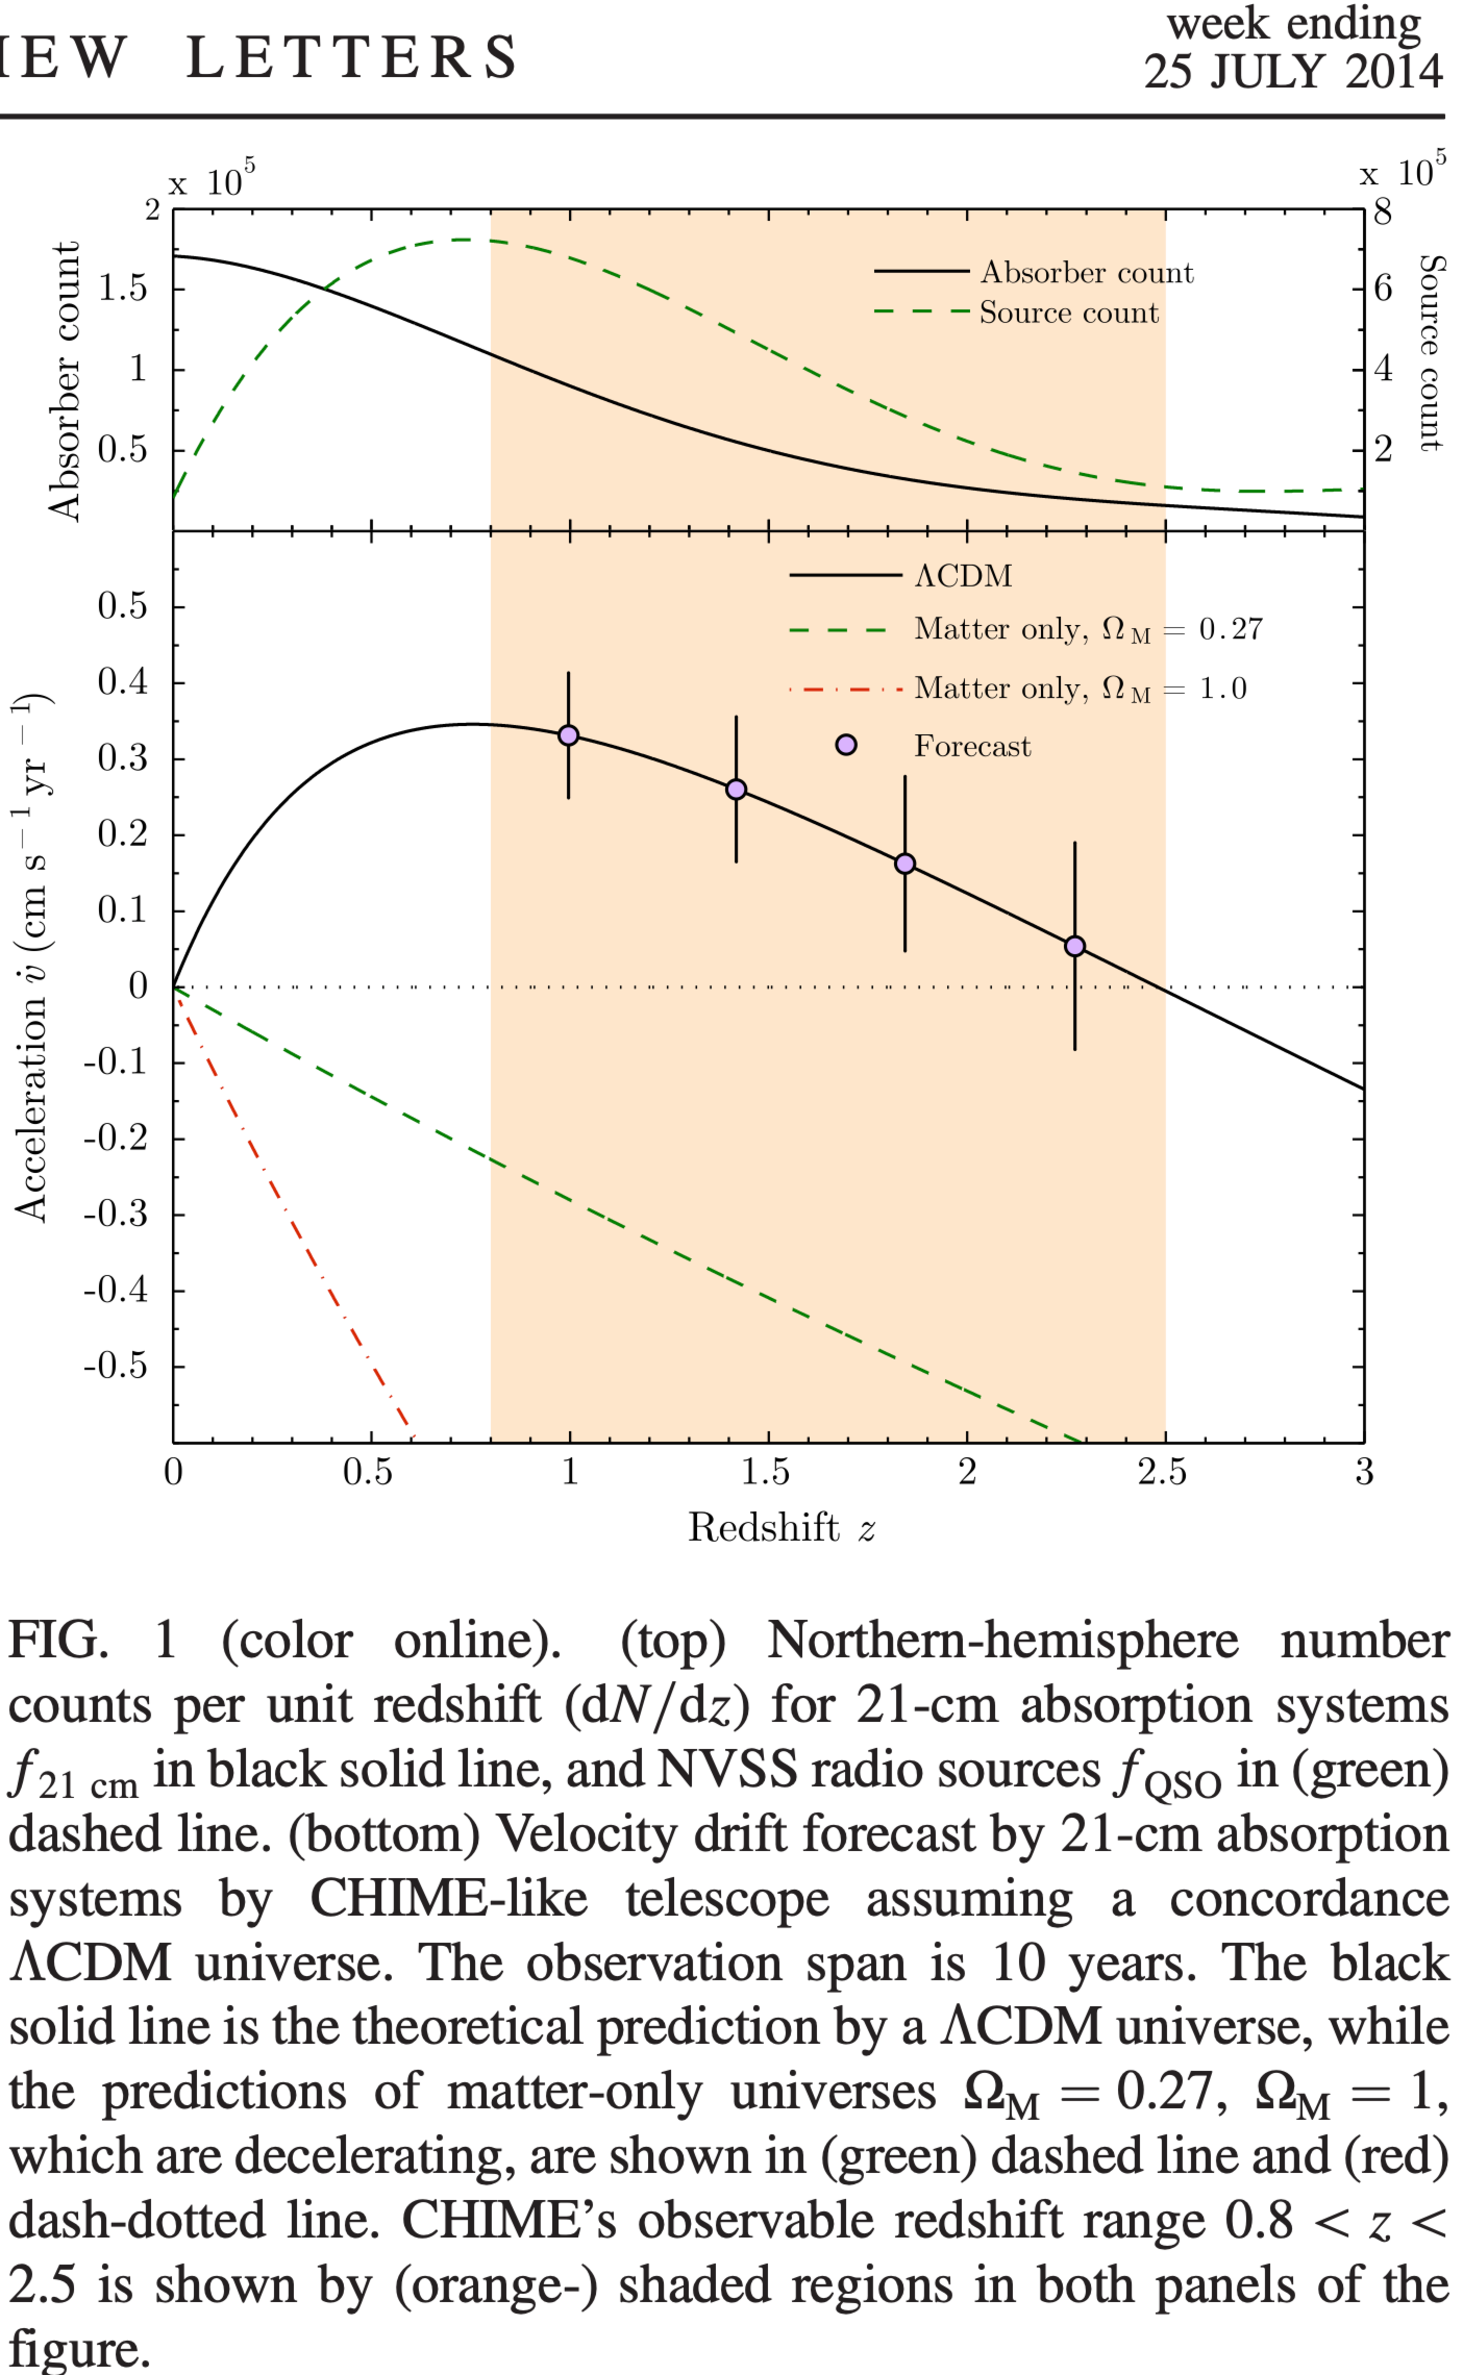
\includegraphics[width=2.0in]{Figures/yuchime.pdf}
\end{center}
  }

  \frame{
    \frametitle{CHIME 21cm upgrade}
    \begin{itemize}
        \item rechannelize all 1024 FRB beams to 4 kHz, about 1km/s
          resolution (James et al)
          \item clever data compression (Arash et al)
        \item earth-sun motion modulates signals by up to 70km/s: look
          for annual doppler drifts
        \item overcomes confusion limit!
          \item CIRADA funded project
    \end{itemize}
  }


  \frame{
%\vspace{-0.5in}
\frametitle{0105-008}
% \hspace{-0.1in}
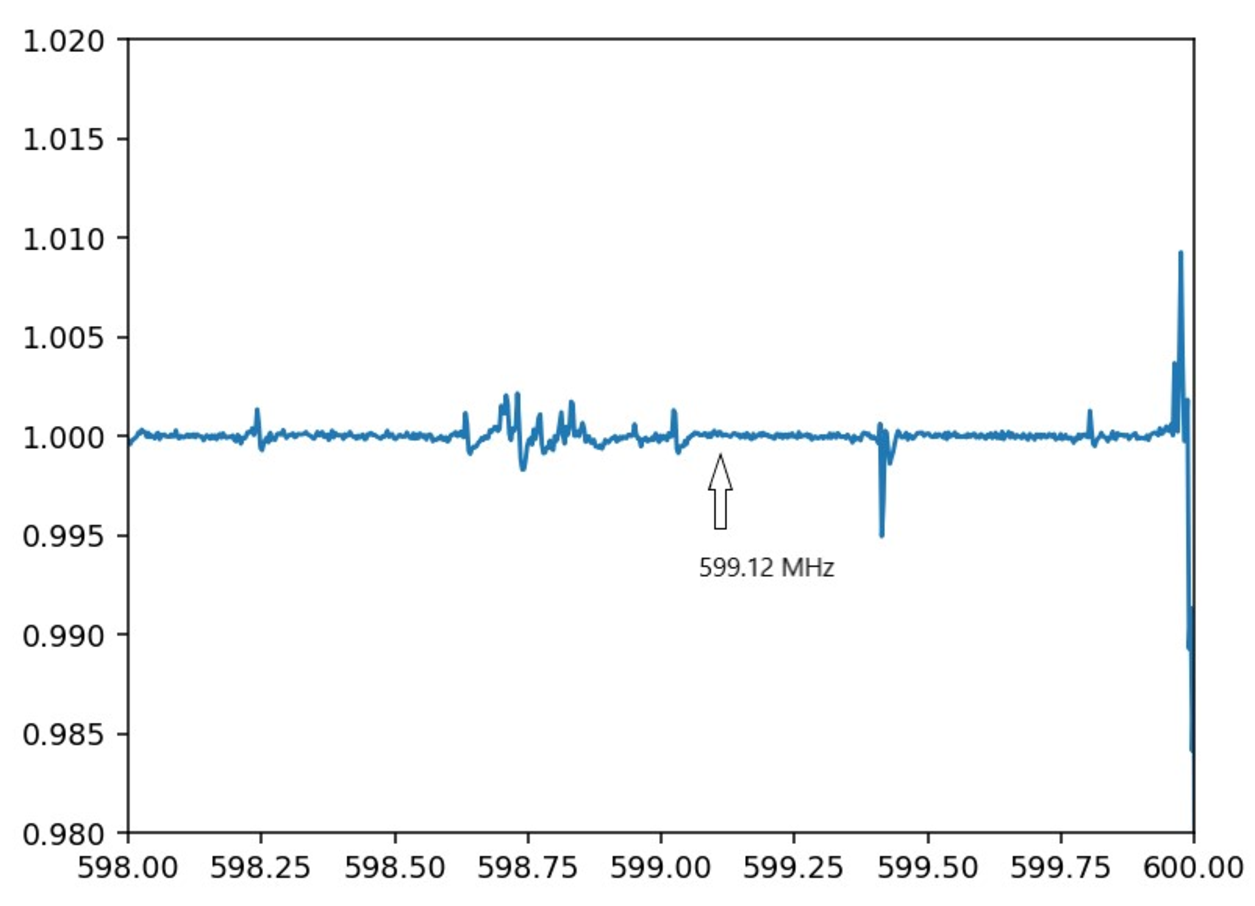
\includegraphics[width=4.2in]{Figures/0105-008.pdf}

  }

  \frame{
\vspace{-0.5in}
    \frametitle{DLA Enigma}
    \begin{itemize}
    \item dominates HI budget in the universe
    \item thought to be key to galaxy formation bayon budget
    \item unclear nature: dwarf galaxies? Giants?
    \item almost all discovered by QSO absorption: blinded by the
      light
    \item most radio sources are optically invisible
    \item CHIME will provide first 'unblinded' DLA sample
    \end{itemize}

  }

  \frame{
\vspace{-0.5in}
    \frametitle{Localization}
    \begin{itemize}
    \item CHIME resolution will limit absorber positions to several arcminutes
    \item potentially confusion limited identification of background source
    \item could localize with CHIME outriggers
    \end{itemize}
  }

  \frame{
\vspace{-0.5in}
    \frametitle{Conclusions}
    \begin{itemize}
    \item CHIME is by far world's fastest radio survey telescope
    \item system seems to work well, und using earth-sun doppler
      motion very stable
    \item testing in progress, currently prognosis optimistic to
      achieve thermal noise limited detections
    \item need to first identify large numbers of absorbers, then
      watch evolution
    \item could start studying absolute clock frequencies for
      posteriority: missed opportunity by Brown and Roberts
    \end{itemize}
  }

\end{document}
